% !TeX TXS-program:compile = txs:///pythontex

\documentclass{article}
\usepackage[utf8]{inputenc}
\usepackage[backend=biber,style=numeric-comp]{biblatex}
\addbibresource{bibliography.bib}
\usepackage{lmodern,microtype,mathtools,amsmath,amsthm,amssymb,icomma,upgreek,xfrac}
\mathtoolsset{mathic}
\usepackage{pythontex}
\usepackage{float}
\usepackage{wrapfig}
\usepackage{graphicx}
\usepackage{caption}
\usepackage{hyperref} % links to gifs and other stuff
\usepackage{subcaption} % captions for many pictures in pharallel
\usepackage{comment} % enables commenting arbitrary amount of text
\usepackage{listings} % for code snippets
\usepackage{xcolor} % for custom colors in code snippets

%define custom colors for code snippets (Colors did not mach what I expected, might need refining later)
\definecolor{vscodeblue}{rgb}{0.16, 0.32, 0.75} % for keywords
\definecolor{vscodegreen}{rgb}{0, 0.6, 0} % for strings
\definecolor{vscodegray}{rgb}{0.5, 0.5, 0.5} % for comments
\definecolor{vscodepurple}{rgb}{0.58, 0, 0.82} % for docstrings
\definecolor{vscodeorange}{rgb}{0.78, 0.39, 0} % for function names
\definecolor{vscodebackground}{rgb}{0.14, 0.16, 0.19} % background color

% configuration for code snippets
\lstset{language=Python,
	basicstyle=\ttfamily\footnotesize\color{white},
    backgroundcolor=\color{vscodebackground},
	keywordstyle=\color{vscodeblue},
	stringstyle=\color{vscodegreen},
	commentstyle=\color{vscodegray},
	morecomment=[s][\color{vscodepurple}]{"""}{"""},
	morecomment=[s][\color{vscodepurple}]{'''}{'''},
	identifierstyle=\color{white},
	classoffset=1, % starting new class for more styles
	morekeywords={np,array,pd,plt},
	keywordstyle=\color{vscodeorange},
	classoffset=0, % revert to default class
	showstringspaces=false,
	breaklines=true,
	frame=none,
	numbers=none,
	numberstyle=\tiny\color{gray},
	tabsize=4,
	captionpos=b,
	escapeinside={(*@}{@*)}, % for escaping to LaTeX inside listing
}

% captions configuration for code snippets
\captionsetup[lstlisting]{font=footnotesize}

% n and z let you specify the tabel  at subsubsection 2.6.3
\begin{pycode}
def function(n):
    z = 1.6181
    a = z
    for i in range(n):
        z = z**2 - 1
    return [f"{z:.4f}",a]
n = 10
\end{pycode}

\title{
	\Huge Holomorphic Dynamics: \\ 
	{\huge an Odyssey from Chaos to Art} 
}
\author{Wojciech Kośnik-Kowalczuk, Olaf Masłowski, Jakub Blukacz}
\date{\today}
\begin{document}
\pagenumbering{arabic}
\maketitle
\thispagestyle{empty}
\begin{figure}[H]
	\centering
	\includegraphics[width=\textwidth]{Utils/article_dependencies/graphic_2.png}
	\caption{\footnotesize $f(z_k) = z_{k-1}^2 -0.8 + 0.156i$}
\end{figure}
\newpage
\thispagestyle{empty}
\tableofcontents
\newpage

\section{Introduction}
Holomorphic dynamics serves as the central theme of this article, with a particular emphasis on the mathematical phenomena known as Julia sets. These sets, arising from the analysis of complex functions, exhibit intricate patterns and fractal geometries. The primary objective is to showcase our computer program visualising these sets and their fractal structures. Furthermore, theoretical basis of Julia sets will be presented, introducing reader to these intricate mathematical objects.

\subsection{Chaos theory}
Although precise examination of chaos theory is outside the scope of this article, in order to give reader a sense of what statement such as \textit{chaotic} mean, we will provide a quote from Edward Lorenz - American mathematician and\\meteorologist:
%\textbf{(wiki/chaos theory na poczatku)}
\begin{quote}
	\textit{"Chaos: When the present determines the future, but the approximate present does not approximately determine the future\cite{zotero-29}."}
\end{quote}
This quote describes sensitivity to initial conditions - the key property of chaotic dynamical systems. Weather is one example of chaotic system.
\begin{center}
	\footnotesize
	\href{run:Utils/article_dependencies/graphic_5.gif}{GIF file presenting rapid changes in Julia sets for \(f(z_{k}) = z_{k-1}^{2} + \alpha\), where \(\alpha\) slowly changes from \(-1\) to \(1\).}

\end{center}

\subsection{Fractal}
%\textbf{(wiki/fractals)}
Fractal is a geometric shape containing detailed structure at arbitrarily small scales, usually having a fractal dimension strictly exceeding the topological dimension. Many fractals appear similar at various scales. This exhibition of similar patterns at increasingly smaller scales is called self-similarity\footnote{\cite{BenoitB.Mandelbrot1983}}.
The term "fractal" was coined by the mathematician Benoît Mandelbrot in 1975. Mandelbrot based it on the Latin frāctus, meaning "broken" or "fractured", and used it to extend the concept of theoretical fractional dimensions to geometric patterns in nature.
Authors disagree on the exact definition of fractal, but most usually elaborate on the basic ideas of self-similarity and the unusual relationship fractals have with the space they are embedded in.
\begin{center}
	\footnotesize
	\href{run:Utils/article_dependencies/graphic_4.gif}{GIF file presenting self-similarities in Mandelbrot set.}
\end{center}

\subsubsection{Real world aplications}
Although the main use for fractals discussed in this article is providing joy for human eye, studying these abstract, chaotic objects may prove useful in analysing chaotic (for example meteorological) models.

\newpage
\section{Julia sets}
This part of article is dedicated to introduce some of concepts crucial to journey of understanding what complex dynamics are. It can be defined study of dynamical systems obtained by iterating a complex analytic mapping. They deal with chaos and order, both in competition and coexistence. They show the transition from one condition to the other and how magnificently complex the transitional region generally is. One of the things many dynamical systems have in common is the competition of several centers for the domination of the plane. A single boundary between territories is seldom the result of this contest. Usually, an unending filigree entanglement and unceasing bargaining for even the smallest areas results\footnote{\cite{Heinz-OttoPeitgen2004}}. %\textbf{(peitgen str 769)}
\\[1\baselineskip]
 Due to programming and showcasing fractals being main focus of this article as well as diffculty of theory behind complex dynamics, said theory will be kept vague, presented in a way that will make it understandable for most STEM students. As Metric Topology course will appear next semester, definitions from that field will not be introduced. \\Unless stated otherwise $z\in\mathbb{C}$.

\subsection{Definition - Holomorphic function}
Let $f$ be complex value function $f:\Omega \rightarrow \mathbb{C}$ on an open set $\Omega$ in the complex plane. $f$ is said to be complex differentiable at $z_{0} \in \mathbb{C}$ if the limit.

\begin{equation}
 \lim_{h\to z_{0}} \frac{f(z_{0} + h) - f(z_{0})}{h} 
\end{equation}

exsist in $\mathbb{C}$. [$\ldots$] We say that $f$ is \textbf{holomorphic} on $\Omega$ if $f$ is complex differentiable at each point of $\Omega$ \footnote{\cite{LarsV.Ahlfors1985}}.	

\subsection{Definition - Extended complex numbers}
\textbf{Extended complex numbers} consist of the complex numbers $\mathbb{C}$ together with $\infty$.
We will denote the set of extended numbers with $\bar{\mathbb{C}}$.
\\
Geometrically, $\bar{\mathbb{C}}$ is referred to as the \textbf{Riemann sphere} (or extended complex plane)\footnote{\cite{ToddRowland}}.

\pagebreak
\subsection{Definition - Fatou sets}
\textit{Let $f(z)$ be a non-constant holomorphic function from the Riemann sphere onto itself. Such functions are precisely the non-constant complex rational functions, that is}
\begin{equation}
	f(z) = \frac{p(z)}{q(z)}
\end{equation}\footnote{\cite{zotero-24}}
Where $p(z)$ and $q(z)$ are complex polynomials. Assume that $p$ and $q$ have no common roots, and at least one has degree larger then $1$. Then there is a finite number of open sets $F_{1},\ldots,F_{r}$, that are left invariant by $f(z)$ (meaning that for $a\in F_{i}, f(a)\in F_{i}$\footnote{\cite{Weisstein}} and are such that:
\begin{enumerate}
	\item The union of the sets $F_{i}$ is dense in the plane.
	\item $f(z)$ behaves in regular and equal way on each of the sets $F_{i}$
\end{enumerate}
These sets $F_{i}$ are the \textbf{Fatou domains} of $f(z)$, and their union is the \textbf{Fatou set} $F(f)$ of $f(z)$.\\
Function $f$ is called the \textbf{iterator}.
\\[1\baselineskip]
\indent{\textbf{Note:}}
\\[1\baselineskip]
The second condition means that the termini of the sequences of iterations generated by the points of $F_{i}$ are either precisely the same set, which is then a finite cycle, or they are finite cycles of circular or annular shaped sets that are lying concentrically. In the first case the cycle is attracting, in the second case it is neutral.

\subsection{Definition - Julia set}
%\textbf{(wiki/Julia set/formal definition)}\\
Let $F(f)$ be Fatou Set. $(F(f))^{c}$ (the compliment of $F(f)$) is the Julia set $J(f)$ of $f(z)$\footnote{\cite{zotero-24}}.

\subsection{Definition - Filled Julia set}
%\textbf{(wiki/filled julia set)}\\
Let $J(f)$ be Julia set. Then union of $J(f)$ and its interior is \textbf{filled Julia set} $K(F)$. If the filled-in Julia set has no interior then the Julia set coincides with the filled-in Julia set\cite{zotero-3}.

\pagebreak
\subsection{Description equivalent to definition 2.4} \label{equivalent}
Julia set can be described in other ways, one of which in particular may be helpful in imagining what Julia set is.

\subsubsection{Alternative description of Julia set}
%\textbf{(wiki/julia set/equivalent descriptions of the Julia set and Fatou set)}\\
If $f$ is an entire function (meaning that it is holomorphic on the whole complex plane), then $J(f)$ is the boundary of the set of points which converge to infinity under iteration\footnote{\cite{Beardon}}.

\subsubsection{Orbit}
%\textbf{(peitgen i inni - chaos and fractals: new frontiers of science (p. 509) - potem wymieniane jako peitgen)}
Let $f_{1}(z) = f(z)$. We define
\begin{equation}
	f_{n+1}(z):=f(f_{n}(z))
\end{equation}
Although formal definition will not be introduced, it will be mentioned that sequence $(f_{1}(z),\ldots,f_{n}(z))$ of iterations of $z$ by $f$ is called \textbf{orbit} through~$z$~\footnote{\cite{Heinz-OttoPeitgen2004}}.\\
We highlight these types of orbits:
\begin{itemize}
	\item \textbf{Constant} - When each iteration gives same value.
	\item \textbf{Periodic} - When values repeat themselves every k iterations.
	\item \textbf{Pre-periodic} - When orbit is not initially periodic, however it becomes one after some k iterations.
	\item \textbf{Chaotic} - When orbit exhbits chaotic behavior.
\end{itemize}

\pagebreak
\subsubsection{Example} \label{Example}
%\textbf{TU ZROBIC TABELKE. MOZNA TEZ ZROBIC W PYTHONIE\\SKRYPT KTORY BEDZIE NUMERYCZNIE SZUKAL WARTOSCI\\$z_{0}$ DLA KTOREJ ITERACJE UCIEKAJA DO NIESKONCZONOSCI\\ (DO DOGADANIA)}\\

\begin{tabular}{c|c|c|c|c|c|c|c}
	$z_{0}$ &
	$f_{1}(z)$ &
	$f_{2}(z)$ &
	$f_{3}(z)$ &
	$\ldots$ &
	$f_{ \py{n-2} }(z)$ &
	$f_{ \py{n-1} }(z)$ &
	$f_{ \py{n} }(z)$  \\ \hline
	\py{function(1)[1]} &
	\py{function(1)[0]} &
	\py{function(2)[0]} & 
	\py{function(3)[0]} & 
	$\ldots$ &
	\py{function(n-2)[0]} & 
	\py{function(n-1)[0]} & 
	\py{function(n)[0]} 

\end{tabular}
\\[2\baselineskip] Let $f(z)=z^{2}-1$ and let us limit oursleves to the real axis of the complex plane. We can see, that for example $f(0)=-1, f_{2}(0)=f(f(0))=0	\\ f(1)=0,\\ f(2)=3, f_{2}(2)=8, f_{3}(2)=63$\\
And $f_{20}(1.618)=0$ but $f_{10}(1.6181)\approx26.755$
\\
In fact it can be shown using numerical approximations that subsequent iterations will diverge to $\infty$ unless $|z| <z_{0}$ where $z_0\approx1.6181$. This means that on the real axis $J(f)=\{-z_{0},z_{0}\}$. As in this instance Julia set $J(f)$ will be connected in $\mathbb{C}$, on real axis filled Julia set $K(f)$ will be equal to $[-z_{0},z_{0}]$

%\textbf{TU TRZEBA DAĆ RENDER $z^{2}-1$}
\begin{figure}[H]
\centering
\includegraphics[scale=0.075]{Utils/article_dependencies/graphic_1.png}
\caption{\footnotesize $z^{2}-1$}
\end{figure}

\newpage
\section{Mandelbrot set}
\begin{figure}[H]
	\centering
	\captionsetup{justification=centering}
	\includegraphics[scale=0.028]{Utils/article_dependencies/graphic_3.png}
	\caption{\footnotesize Mandelbrot set}
\end{figure}
Perhaps the most famous fractal structures are those of the Mandlebrot set \footnote{\cite{Heinz-OttoPeitgen2004}}. It is not authors' intention to present underlying theory behind the Mandelbrot set. However, we would like to discuss relations it has with the Julia set. We will define the Mandelbrot set as following:

\subsection{Definition - mandelbrot set}
The Mandelbrot set, denoted as $M$, is set of values $c\in\mathbb{C}$ for which function $f_{c}:\mathbb{C} \rightarrow \mathbb{C},\\f_{c}(z)=z^{2}+c$ does not diverge to infinity when iterated starting at $z=0$\footnote{\cite{Weissteina}}.
\\[2\baselineskip]
It is simple observation, that iterating $f_{c}$ as described above is equivalent to iterating $f(0)$ (where $f(z)=z^{2}+c$).

\pagebreak
\subsection{\texorpdfstring{Link between $J(f)$ and $M$}{Link between J(f) and M}} \label{JandM}
Another way to define the Mandelbrot set is by describing it with corresponding Julia set:\\
Let $f(z)=z^{2}+c$. The Mandelbrot set is the subset of the space of parameters $c$ for which the Julia set $J(f)$ forms a connected set.

\subsection{The mandelbrot set as a roadmap for Julia sets}
The Mandelbrot set is a visualization of the structural dichotomy of Julia sets for the quadratic iterator. Let us have a look at the figure above.	 We choose as particular c-values the major branch points of these dendrites (see arrows). For each of these 5 c-values we compute the associated Julia set, displayed in the lower part of the figure. We observe a striking resemblance in the structures and the combinatorics of the dendritic structures in the Mandelbrot set and the Julia sets. The geometry of these Julia sets is also visible in the Mandelbrot set when magnified appropriately at the corresponding parameter values. In this sense it is a visual table of content of the book of Julia sets.
\begin{figure}[H]
	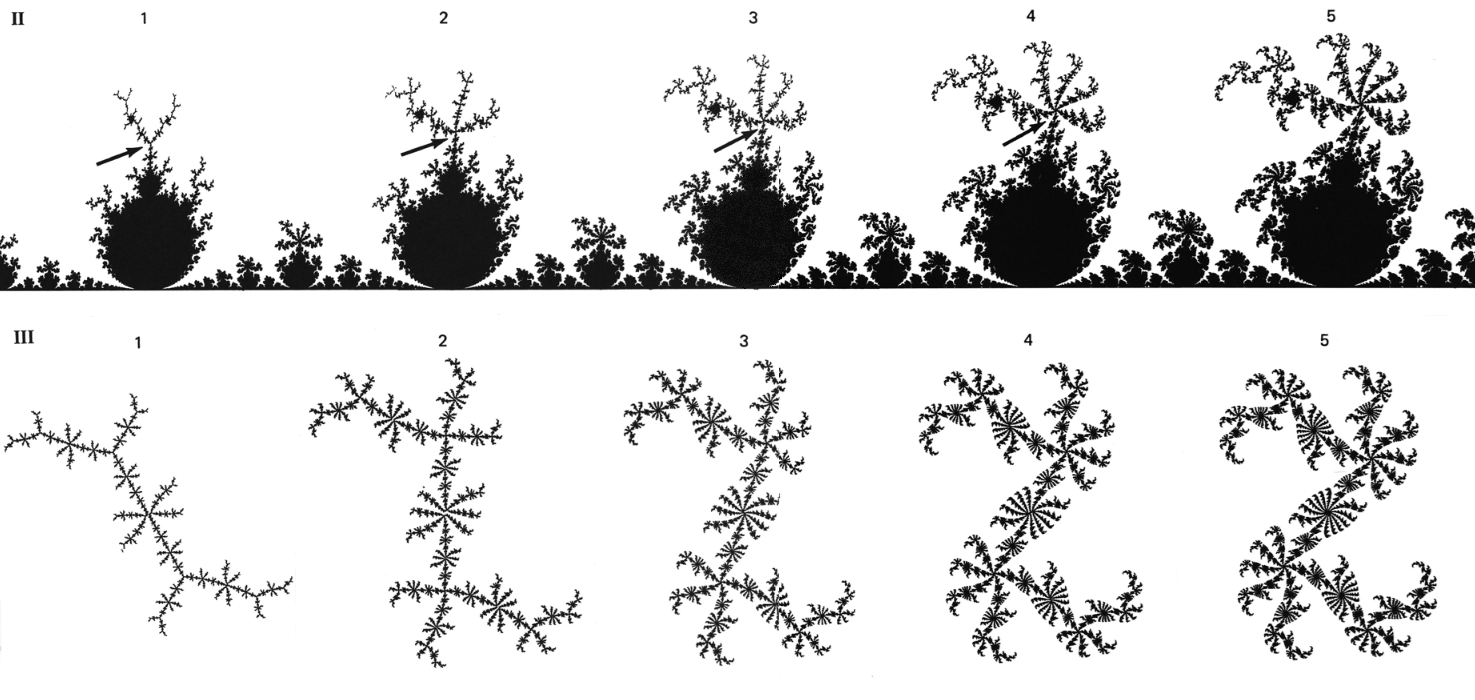
\includegraphics[width=\linewidth]{Utils/article_dependencies/Picture_for_5_3.png}
	\caption{\footnotesize \cite{Heinz-OttoPeitgen2004}, page 876-878}
\end{figure}

\newpage

\section{Implementation in Python}

\begin{center}
	\scriptsize(NOTE: Certain terminology in this section might differ from previous text for clarity, as it could otherwise lead to ambiguity in context of programming. If text feels incoherent and misleading, pleas let us now to so we can improve upon it)
\end{center}

\subsection{Introduction}
As we mentioned before, the main objective of this project is to implement an easy to use fractal renderer for educational purposes. Such tool lets user experiment with mentioned sets and study their behavior in an intuitive visual way. This graphic representation of such sets stands out as a particularly intriguing aspect of holomorphic dynamics. Julia sets and related ones seem to take an amazingly natural and organic shapes, potentially prompting the reader to a deeper exploration of epistemological Platonism within the realm of mathematics. 
\\[1\baselineskip]
Unfortunately, when it comes to implementing most mathematical concepts numerically it's necessary to approximate the solution.
To visualize those sets we will map their orbits to the color space. This will allow us to see the structure of the set. The mapping uses the number of iterations it took for the orbit to escape the circle of a given radius. The color of the pixel is then determined by the number of iterations it took. In addition we will approximate the convergence of the orbit by calculating an arbitrary number of iterations, a value derived through meticulous testing of numerical effectiveness and optimization (in most cases set at 256, as it provides adequate results and allows for the utilization of the uint8 datatype).
\\[1\baselineskip]
Why is such approximation is valid? We can present it by simplifying the problem to a much more intuitive space $\mathbb{R}$. Iterating function $f(x_k) = x_{k-1}^2$, where $x \in \mathbb{R}$ will showcase the behavior of orbits:
\\[1\baselineskip]
For values of $x$ more than $1$, the orbit will escape to infinity. \\ 
For $x=1$ the orbit will stay at $1$. \\
For $x$ between $-1$ and $1$ the orbit will converge to $0$. \\
For $x$ less than $-1$ the orbit will also escape to infinity.
\\
More on that in section \hyperref[equivalent]{2.6}
\\[1\baselineskip]
In this example we can call $0$ and $1$ fixed points of our iterative function. The point $0$ is identified as an attractive fixed point, due to the fact that orbits starting in its vicinity converge towards it. Point $1$ is a repulsive fixed point, owing to the fact that orbits around it diverge from it.
\\[1\baselineskip]
Values in the interval $[-1,1]$ will not escape to infinity and thus constitute our set (filled Julia set). In contrast values outside of this interval generate unbounded orbits, and are thus not included in the set.\\
\pagebreak
This behavior seems intuitively justified by recognizing that $1$ is an identity element for multiplication over $\mathbb{R}$, and so it's natural for orbits to maintain their stationary state at $1$. The operation of squaring (that is multiplication of a number by itself) ensures that values below $0$ will be mirrored after the initial iteration to the positive side of the number line, so we can expect similar behavior to positive numbers, after the first iteration. Finally value of $0$ being less than $1$ (and $-1$ in the mirrored domain), is anticipated to attract nearby orbits.
\\[1\baselineskip]
This example is very straightforward, so let's introduce complexity by modifying our function. We can use example from \hyperref[Example]{section 2.6.3}: $f(x) = x^2 - 1$. This small adjustment can provide us with examples of more interesting orbit behaviors.
\\[1\baselineskip]
For $x=1$ the orbit will transition from $f(1) = 0$ to $f(0) = -1$ and returning to $f(-1) = 0$. Such orbit is called periodic.
\\
Orbits initializing between $-1$ and $1$ are incorporated in our set. Moreover, orbits starting in proximity to this interval tend to fall into it during initial iterations, thus being included in the set as well.
\\
Many orbits will exhibit seemingly chaotic behavior before stabilizing. For instance, starting from $0.5$, the sequence progresses as follows:
\\
$0.5 \rightarrow -0.75 \rightarrow -0.4375 \rightarrow -0.808594 \rightarrow -0.346176 \rightarrow -0.880162 \rightarrow$ \\
$\rightarrow -0.225315 \rightarrow -0.949233 \rightarrow -0.0989567 \rightarrow -0.990208 \rightarrow -0.0194881 \rightarrow$ \\ $\rightarrow -0.99962 \rightarrow -0.000759856 \rightarrow -0.999999$ and so on.
\\
Initially, the orbit appears chaotic, but in the limit, it stabilizes as a periodically stable orbit oscillating between $0$ and $-1$.
\\
Simple subtraction of $1$ from the previous function has made the orbit's behavior far more complex. Extending this analysis from the real axis to the complex plane and broadening our function $f(x)$ to the whole family of iterative functions like $f(z_k) = z_{k-1}^2 + c$, where $z$ is a complex variable and $c$ is a complex constant, we can find infinitely intricate behavior of orbits. Plotting them as a color map will allow us to see the structure of those unimaginably complex sets.
\\[1\baselineskip]
As we observed in simpler examples, the divergence of orbits originating at points equal or beyond $1$ from the origin of real axis is intuitively anticipated and this expectation is readily justified. This principle seamlessly extends to the complex plane. It is proven, that within the Mandelbrot set any orbit exceeding a radius of 2 is guaranteed to diverge to infinity. This threshold of 2 for divergence provides equally useful results to aproximate Julia sets, demonstrating its utility in visualization across numerous tests. However, if we adjust our definition of Julia sets to include, for example trigonometric functions, exemplified by $f(z_k) = \sin(z_{k-1}) \cdot c$, the radius of divergence will need to be adjusted.

\pagebreak
\subsection{Basic Renderer}

Armed with the knowledge gained we can now proceed to implement the fractal renderer. Following libraries will be essential to utilize:

\begin{lstlisting}[language=Python, caption=Essential libraries]
	
	import numpy as np					# For array manipulation
	from PIL import Image   			# For image processing
	import matplotlib.pyplot as plt		# For applying colormaps
	from sympy import sympify, lambdify, symbols    # For symbolic mathematics
	
\end{lstlisting}

\begin{center}
	\scriptsize (Note: Code from snippets included in paper are available as executable noteboooks in main catalog of this repository)
\end{center}

\noindent{Additionally few other libraries are employed for final renderer. However the scope of this paper will be centered around explaining basic functionality of renderer.}
\\[1\baselineskip]
A critical component to begin with is building a function computing the orbits for a given sympy expression, this is crucial for determining membership in Julia set. For that we'll need to initialize several constants:

\begin{lstlisting}[language=Python, caption=Declaring constants]
	
	max_iterations = 256
	max_magnitude = 2
	
	# initial definition of attractor function
	attractor_str = 'z^2 + const'  
	
	# example value of complex xonstant
	const = 0.4 + 0.4j
	
	# resolution of output file in pixels
	res_w, res_h = 1000, 1000  
	
	# complex plane range to be rendered
	re_min, re_max, im_min, im_max = -2, 2, -2, 2  
	
\end{lstlisting}

\noindent{Subsequently we can compute our function, using sympy symbolic abilities, to be a callable object compatible with numpy's vectorized operations:}

\begin{lstlisting}[language=Python, caption=Preparing callable iterator]
	
	# lambda like callable
	# compatible with numpy vectorized operations
	attractor = lambda x1, x2: lambdify(symbols('z const'), \
	sympify(attractor_str), 'numpy')(x1, x2)
	
\end{lstlisting}
\pagebreak

\noindent{Finally we can write our function, utilizing vectorized operations:}

\begin{lstlisting}[language=Python, caption=Function to check if in Julia set]
	
	def if_in_Julia_set(z_arr: np.array, data: np.array) -> None:
	'''
	Calculates if Julia set contains a given point.
	Uses sympy expression for attractor function.
	
	Operates on passed data array !!!
	
	Parameters:
	- z_arr: array of complex numbers corresponding to pixels (np.array)
	- data: array to populate with iterations till exceeding max_magnitude or max_iteration if not exceeded (np.array)
	'''
	
	# initialize helper array
	not_exceeding = np.ones_like(data, dtype=bool)
	
	# iterate till exceeding max_magnitude or max_iteration if not exceeded
	for _ in np.arange(max_iterations):
	
	# evaluate attractor function for relevant pixels, for current iteration
	z_arr = np.where(not_exceeding, attractor(z_arr, const), z_arr)
	
	# mark points exceeding max_magnitude
	not_exceeding = ~(np.abs(z_arr) > max_magnitude)
	
	# update data
	data[not_exceeding] += 1
	
	# adjust data to prevent uint8 overflow
	data[data == max_iterations] = max_iterations - 1
	
\end{lstlisting}

\pagebreak
\noindent{Now let's introduce the rendering function:}

\begin{lstlisting}[language=Python, caption=Renderer]
	
	def render_vectorwise(data: np.array) -> np.array:
	'''Renders Julia set as numpy array'''
	
	# initialize array of complex numbers corresponding to pixels
	# np.linspace creates array of evenly spaced numbers over resolution range
	# np.newaxis extends array by new axis (column vector)
	# data contains complex numbers corresponding to pixels
	z_arr = np.linspace(re_min, re_max, res_w) + 1j \
	* np.linspace(im_min, im_max, res_h)[:, np.newaxis]
	
	# calculate orbits for given origins array
	if_in_Julia_set(z_arr, data)
	
\end{lstlisting}

\noindent{Remembering that the Julia set is the border between bounded and divergent orbits, we can plot our calculations using color maps that will show not only divergence, but also the amount of iterations it took the orbit to exceed our maximum magnitude of 2 and save it as a PNG image:}

\begin{lstlisting}[language=Python, caption=Final PNG function]
	
	def render(color_map: str = "twilight_shifted") -> None:
	'''Renders Julia set into .png file'''
	
	# initialize image
	image = Image.new('RGB', (res_h, res_w))
	
	# initialize data
	data = np.zeros((res_h, res_w), dtype=np.uint8)
	
	# create data
	render_vectorwise(data)
	
	# map data to colors
	# normalize orbits
	normalized_orbits = data / max_iterations
	# get colormap
	cmap = plt.get_cmap(color_map)
	# map orbits
	pixels = (cmap(normalized_orbits)[:,:,:3] * 255) \
	.astype(np.uint8) # excluding alpha channel
	
	# save data to image
	image = Image.fromarray(pixels, 'RGB')
	image.save( \
	f"Julia_set_{attractor_str}_res_{res_w}x{res_h}.png")
	
\end{lstlisting}

\noindent{And last but not least, let's plot it!}

\begin{lstlisting}[language=Python, caption=Execution]
	
	render()
	
\end{lstlisting}

\begin{figure}[H]
	\includegraphics[width=\linewidth]{Utils/article_dependencies/Implementation_chapter/render_1.png}
	\caption{\footnotesize Our first render}
\end{figure}

\newpage
\subsection{Visual Analysis}

Now that we have developed a tool capable of rendering visual representations of Julia sets, we can conduct a visual analysis of these mathematical entities. A key observation to start from is that varying the \texttt{const} argument yields different fractal patterns.
\\
For instance:

\begin{figure}[H]
	\centering
	% First Row
	\begin{subfigure}[b]{0.45\linewidth}
		\includegraphics[width=\linewidth]{Utils/article_dependencies/Implementation_chapter/render_2.png}
		\caption{\footnotesize $const = 0.285 + 0.01j$}
	\end{subfigure}
	\hfill
	\hfill
	\begin{subfigure}[b]{0.45\linewidth}
		\includegraphics[width=\linewidth]{Utils/article_dependencies/Implementation_chapter/render_3.png}
		\caption{\footnotesize $const = -0.835 - 0.2321j$}
	\end{subfigure}
	
	% Second Row
	\begin{subfigure}[b]{0.45\linewidth}
		\includegraphics[width=\linewidth]{Utils/article_dependencies/Implementation_chapter/render_4.png}
		\caption{\footnotesize $const = 0.35 + 0.35j$}
	\end{subfigure}
	\hfill
	\begin{subfigure}[b]{0.45\linewidth}
		\includegraphics[width=\linewidth]{Utils/article_dependencies/Implementation_chapter/render_5.png}
		\caption{\footnotesize $const = -0.4 + 0.6j$}
	\end{subfigure}
	
	\caption{Visualizations of Julia sets for different values of $const$.}
\end{figure}
\pagebreak

\noindent{Furthermore it's noteworthy that in the vicinity of the Mandelbrot set's boundary we can find most visually intricate patterns of Julia sets. This observation stems from the relationship between the two explained earlier. Just to mention, the Mandelbrot set is generated by iterative function, that takes \(z=0\) as a starting argument and varying the \texttt{const} value. Hence, for a given \texttt{const} value the orbit of Julia set is the same as for Mandelbrot set. Consequently for values inside the Mandelbrot set Julia sets won't be as visually stimulating as near it's boundary. The impression will be similar for values distant from the Mandelbrot set's boundary:}

\begin{figure}[H]
	\centering
	% first image
	\begin{minipage}{0.45\textwidth}
		\centering
		
\includegraphics[width=\linewidth]{Utils/article_dependencies/Implementation_chapter/render_6.png}
		\caption{\footnotesize $const = 0$}
		\label{fig:render6}
	\end{minipage}
	\hfill
	% second image
	\begin{minipage}{0.45\textwidth}
		\centering
		
\includegraphics[width=\linewidth]{Utils/article_dependencies/Implementation_chapter/render_7.png}
		\caption{\footnotesize $const = 10 + 10j$}
		\label{fig:render7}
	\end{minipage}
\end{figure}

\noindent{Most fascinating geometries can be discovered near the boundary of the Mandelbrot set. Utilizing the near-circular, cardioid-like shape of the Mandelbrot, we can generate captivating plots for values of \texttt{const} which magnitude is approximately equal to radius of the boundary. To enhance ease of exploring those shapes and underscore the dynamic nature of the subject, we can animate it into a single GIF file.}
\\[1\baselineskip]
For that we'll need to adjust our code by adding one more outer loop generating subsequent images to be concatenated to a single GIF file.
\pagebreak

\noindent{To accomodate the dynamic visualization for varying value of \texttt{const} parameter, we refine the existing function for determining Julia set membership:}

\begin{lstlisting}[language=Python, caption=if\_in\_Julia\_set adjustments for GIF format]
	
	def if_in_Julia_set(z_arr: np.array, data: np.array, \
	curr_const: complex=None):
	"""
	Calculates if Julia set contains a given point.
	Uses sympy expression for attractor function.
	
	Operates on passed data array !!!
	
	Parameters:
	- z_arr: array of complex numbers corresponding to pixels (np.array)
	- data: array to populate with iterations till exceeding max_magnitude or max_iteration if not exceeded (np.array)
	- curr_const: current value of complex constant, if not given global const value will be utilized (complex)
	"""
	
	# set value of current const if given
	if not curr_const: curr_const = const
	# ADJUSTMENT FOR ANIMATED RENDERS ^^^
	
	# initialize helper array
	not_exceeding = np.ones_like(data, dtype=bool)
	
	# iterate till exceeding max_magnitude or max_iteration if not exceeded
	for _ in np.arange(max_iterations):
	
	# evaluate attractor function for relevant pixels, for current iteration
	z_arr = np.where(not_exceeding, attractor(z_arr, curr_const), z_arr)
	
	# mark points exceeding max_magnitude
	not_exceeding = ~(np.abs(z_arr) > max_magnitude)
	
	# update data
	data[not_exceeding] += 1
	
	# adjust data to prevent uint8 overflow
	data[data == max_iterations] = max_iterations-1
	
\end{lstlisting}

\pagebreak
\noindent{We will also need to adjust the rendering function to return an \texttt{Image} object, but to ensure simplicity and readability of the existing code, we can simply design it from scratch:}

\begin{lstlisting}[language=Python, caption=Frame rendering function]
	
	def render_frame(current_const: complex=0+0j, \
	color_map: str="twilight_shifted") \
	-> Image:
	"""Renders Julia set animation frame as numpy array"""	
	
	# initialize data array
	data = np.zeros((res_h, res_w), dtype=np.uint8)
	
	# initialize orbits
	z_arr = np.linspace(re_min, re_max, res_w) + 1j \
	* np.linspace(im_max, im_min, res_h)[:, np.newaxis]
	
	# calculate orbits based on their origins
	if_in_Julia_set(z_arr, data, current_const)
	
	# map data to colors
	# normalize orbits
	normalized_orbits = data / max_iterations
	# get colormap
	cmap = plt.colormaps[color_map]
	# map orbits
	pixels = (cmap(normalized_orbits)[:, :, :3] \
	* max_iterations).astype(np.uint8)
	
	# return image
	return Image.fromarray(pixels, 'RGB')
	
\end{lstlisting}

\pagebreak
\noindent{Finally, we can cover it all up with an outer layer that is a loop through frames that will compute consecutive values of \texttt{const} and call the above function for render image, to concatenate them all into a single GIF file:}

\begin{lstlisting}[language=Python, caption=Creation of GIF file]
	
	def render_gif(frames_amount: int=200, frame_duration: int=25):
	'''Renders Julia sets visualizations and saves them into GIF'''
	
	# approximated radius of carioic shape of Mandelbrot set
	magnitude = 0.8
	
	# const value list ( exp(i*alpha), where alpha e [0, 2Pi] )
	const_values = magnitude * np.exp(1j * np.linspace(0, 2 * np.pi, frames_amount))
	
	# loop through frames
	frames = []
	for i in range(frames_amount):
	
	# render frame for current constant
	frames.append(render_frame(const_values[i]))
	
	# save image to GIF file
	frames[0].save(f"Julia_set_{attractor_str}_res_{res_w}x{res_h}.gif", format='GIF', 
	append_images=frames[1:], save_all=True, duration=frame_duration, loop=0)
	
\end{lstlisting}

\noindent{Culminating it all up, the only thing to do is to execute the rendering of our animation!}

\begin{lstlisting}[language=Python, caption=Execution of GIF renderer]
	
	render_gif()
	
\end{lstlisting}

\begin{center}
	\footnotesize
	\href{run:Utils/article_dependencies/Implementation_chapter/render_8.gif}{Our first animated visualization!}
\end{center}

\newpage
\subsection{Fractals and Their Non-Intuitive Dimensionality}

\noindent{One last thing I wanted to mention in this paper is the dimensionality of fractals. Though it was covered in \texttt{1.2}, I want to revisit the topic now that we have a tool to visualize it. When it comes to these unusual mathematical entities it starts to make sense to talk about fractional dimensions (Minkowski-Bouligand dimension, Hausdorff dimension, etc,..). At first glance the notion of fractional dimensions may seem perplexing, yet it will become more coherent after short explanation.}
\\
These shapes, as our examples have shown, can exhibit infinitely intricate boundary and so have an infinite length in a finite area, essentially bridging the gap between conventional dimensions. It can be achived by staying irregular at arbitrary scale. This behavior can be seen in the graphic below:

\begin{center}
	\footnotesize
	\href{run:Utils/article_dependencies/Implementation_chapter/render_9.gif}{Mandelbrot set zoom effect}
	\\
	\scriptsize(Note: The code generating such a zoom effect on the Mandelbrot set is pretty straightforward and will be ommited here for brevity. However I remind the reader that all renders and the codebase to create them is contained in this repository and can be easily explored)
\end{center}

\noindent{One of the more difficult challenges with computing such renders is that for really deep zooms the fine line between divergent and non divergent orbits can be overwhelmed by ever so slowly diverging orbits. Currently we determine divergence by analyzing first $256$ iterations of the function, but to visualize (even if only approximately) infinite complexity we'll need to adjust this parameter and to do so we might need to refine the types we're using, from \texttt{uint8} (capable of storing $256$ values) to \texttt{uint16} (capable of storing $65 536$ values).}
\pagebreak

\noindent{Once again we will need to refine the existing function for determining Julia set membership by adding \texttt{curr\_iter} parameter, that controls how many iterations infer divergence:}

\begin{lstlisting}[language=Python, caption=Another adjustment to if\_in\_Julia\_set unction]
	
	def if_in_Julia_set(z_arr: np.array, data: np.array, \
	curr_const: complex=None, \
	curr_iter: int=256):
	'''
	Calculates if Julia set contains a given point.
	Uses sympy expression for attractor function.
	
	Operates on passed data array !!!
	
	Parameters:
	- z_arr: array of complex numbers corresponding to pixels (np.array)
	- data: array to populate with iterations till exceeding max_magnitude or max_iteration if not exceeded (np.array)
	- curr_const: current value of complex constant, if not given global const value will be utilized (complex)
	- curr_iter: current number of iterations to compute (int)
	'''
	
	# set value of current const if given
	if not curr_const: curr_const = const
	
	# set current number of iterations to compute
	max_iterations = curr_iter
	# ADJUSTMENT FOR ANIMATED RENDERS ^^^
	
	# initialize helper array
	not_exceeding = np.ones_like(data, dtype=bool)
	
	# iterate till exceeding max_magnitude or max_iteration if not exceeded 
	for _ in np.arange(max_iterations):
	
	# evaluate attractor function for relevant pixels, for current iteration
	z_arr = np.where(not_exceeding, attractor(z_arr, curr_const), z_arr)
	
	# mark points exceeding max_magnitude
	not_exceeding = ~(np.abs(z_arr) > max_magnitude)
	
	# update data
	data[not_exceeding] += 1
	
	# break the loop if all elements exceeded given magnitude
	if not any(not_exceeding): break
	
	# adjust data to prevent uint8 overflow
	data[data == max_iterations] = max_iterations-1
	
\end{lstlisting}
\pagebreak

\noindent{Additionally, we need to adjust our \texttt{render\_frame} function to operate on a more capacious data type, \texttt{uint16}:}

\begin{lstlisting}[language=Python, caption=Frame rendering function utilizing uint16 data type]
	
	def render_frame_uint16(current_iterations_max:int=256, \
	color_map:str="twilight_shifted") \
	-> Image:
	'''
	Renders Julia set for given number of iterations as numpy array
	'''
	
	data = np.zeros((res_h, res_w), dtype=np.uint16)
	# TYPE CHANGE HERE ^^^^^^^^^^^^^^^^^^^^^^^^^^^^^
	
	z_arr = np.linspace(re_min, re_max, res_w) + 1j \
	* np.linspace(im_max, im_min, res_h)[:, np.newaxis]
	
	# calculate orbits
	if_in_Julia_set(z_arr, data, const, current_iterations_max)
	
	# map data to colors
	# normalize orbits 
	normalized_orbits = data / current_iterations_max
	# get colormap
	cmap = plt.colormaps[color_map]
	# map orbits
	pixels = (cmap(normalized_orbits)[:,:,:3] \
	* 255).astype(np.uint8)
	# DID NOT CHANGE TYPE HERE ^^^^^
	
	# return image
	return Image.fromarray(pixels, 'RGB')
	
\end{lstlisting}

\pagebreak
\noindent{Last but not least, we can rewrite \texttt{render\_gif} to update value of \texttt{max\_iter} instead of \texttt{const}. We will update it logarithmically, because changes at the beginning of the spectrum are more visible for human eye, than changes happening far into the large numbers of iterations regime:}

\begin{lstlisting}[language=Python, caption=Zoom effect rendering function]
	
	def render_gif(frames_amount:int=500, frame_duration:int=25, \
	log_2_max_iter_start:int=4, \
	log_2_max_iter_end:int=12) -> None:
	
	# spread vaalues of max iter logarithmically to better see first elements
	# log_2_max_iter_start  - start of logarythmic scale (2^log_...)
	# log_2_max_iter_end    - end of logarythmic scale (2^log_...)
	# frames_amount         - how many elements to generate
	# False                 - not including log_2_max_iter_end as element (ensures not getting to limit of uint16 data type)
	# int                   - casts elements too ints
	max_iter_values = np.logspace(log_2_max_iter_start, \
	log_2_max_iter_end, \
	frames_amount, \
	False, \
	2, \
	int)
	
	# loop through frames
	frames = []
	for i in range(frames_amount):
	
	# render frame for current number of iterations to compute
	frames.append(render_frame_uint16(max_iter_values[i]))
	
	frames[0].save(f"Julia_set_{attractor_str}_res_{res_w}x{res_h}.gif", \
	format='GIF', \
	append_images=frames[1:], \
	save_all=True, \
	duration=frame_duration, \
	loop=0)
	
\end{lstlisting}

\noindent{And run!}

\begin{lstlisting}[language=Python, caption=Execute zoom effect render]
	
	render_gif()
	
\end{lstlisting}

\begin{center}
	\footnotesize
	\href{run:Utils/article_dependencies/Implementation_chapter/render_10.gif}{Visualisation of infinite complexity of the sets border}
\end{center}

\newpage

\section{Afterwords}

It is our  sincere hope that this exploration of the mesmerizing world of fractals was as engaging and as captivating for the reader as for the authors of this paper. For those whose curiosity remains unquenched, we will end this paper with few more examples of those marvellous visuals and leave the reader with tools to dive deeper into the realm of fractals.
\\[1\baselineskip]
This repository contains a codebase with a comprehensive suite of tools designed for fractal generation, with different parameters to experiment with. The repository is an ongoing project and gets updates on a weekly basis, but it already contains a rich collection of functionalities. From color mapping's operations to creating visuals based on for example; polynomial, exponential, trigonometric, functions, and vastly more. We wholeheartedly encourage the reader to pause and dive into the creative process of fractal exploration.
\\[1\baselineskip]
Your insights, ideas, suggestions and recommendations are highly valued. If you are inspired to code with us, have recommendations to share, or wish to propose improvements, we eagerly invite you to submit a pull request or reach out to us via email at:
\begin{center}
	\href{mailto:wojciech.kosnik.kowalczuk@gmail.com}{wojciech.kosnik.kowalczuk@gmail.com}
\end{center}

\pagebreak
\subsection{Honorable mentions}

\begin{figure}[H]
	\includegraphics[width=\linewidth]{Utils/article_dependencies/Honorable_mentions/1.png}
\end{figure}

\begin{figure}[H]
	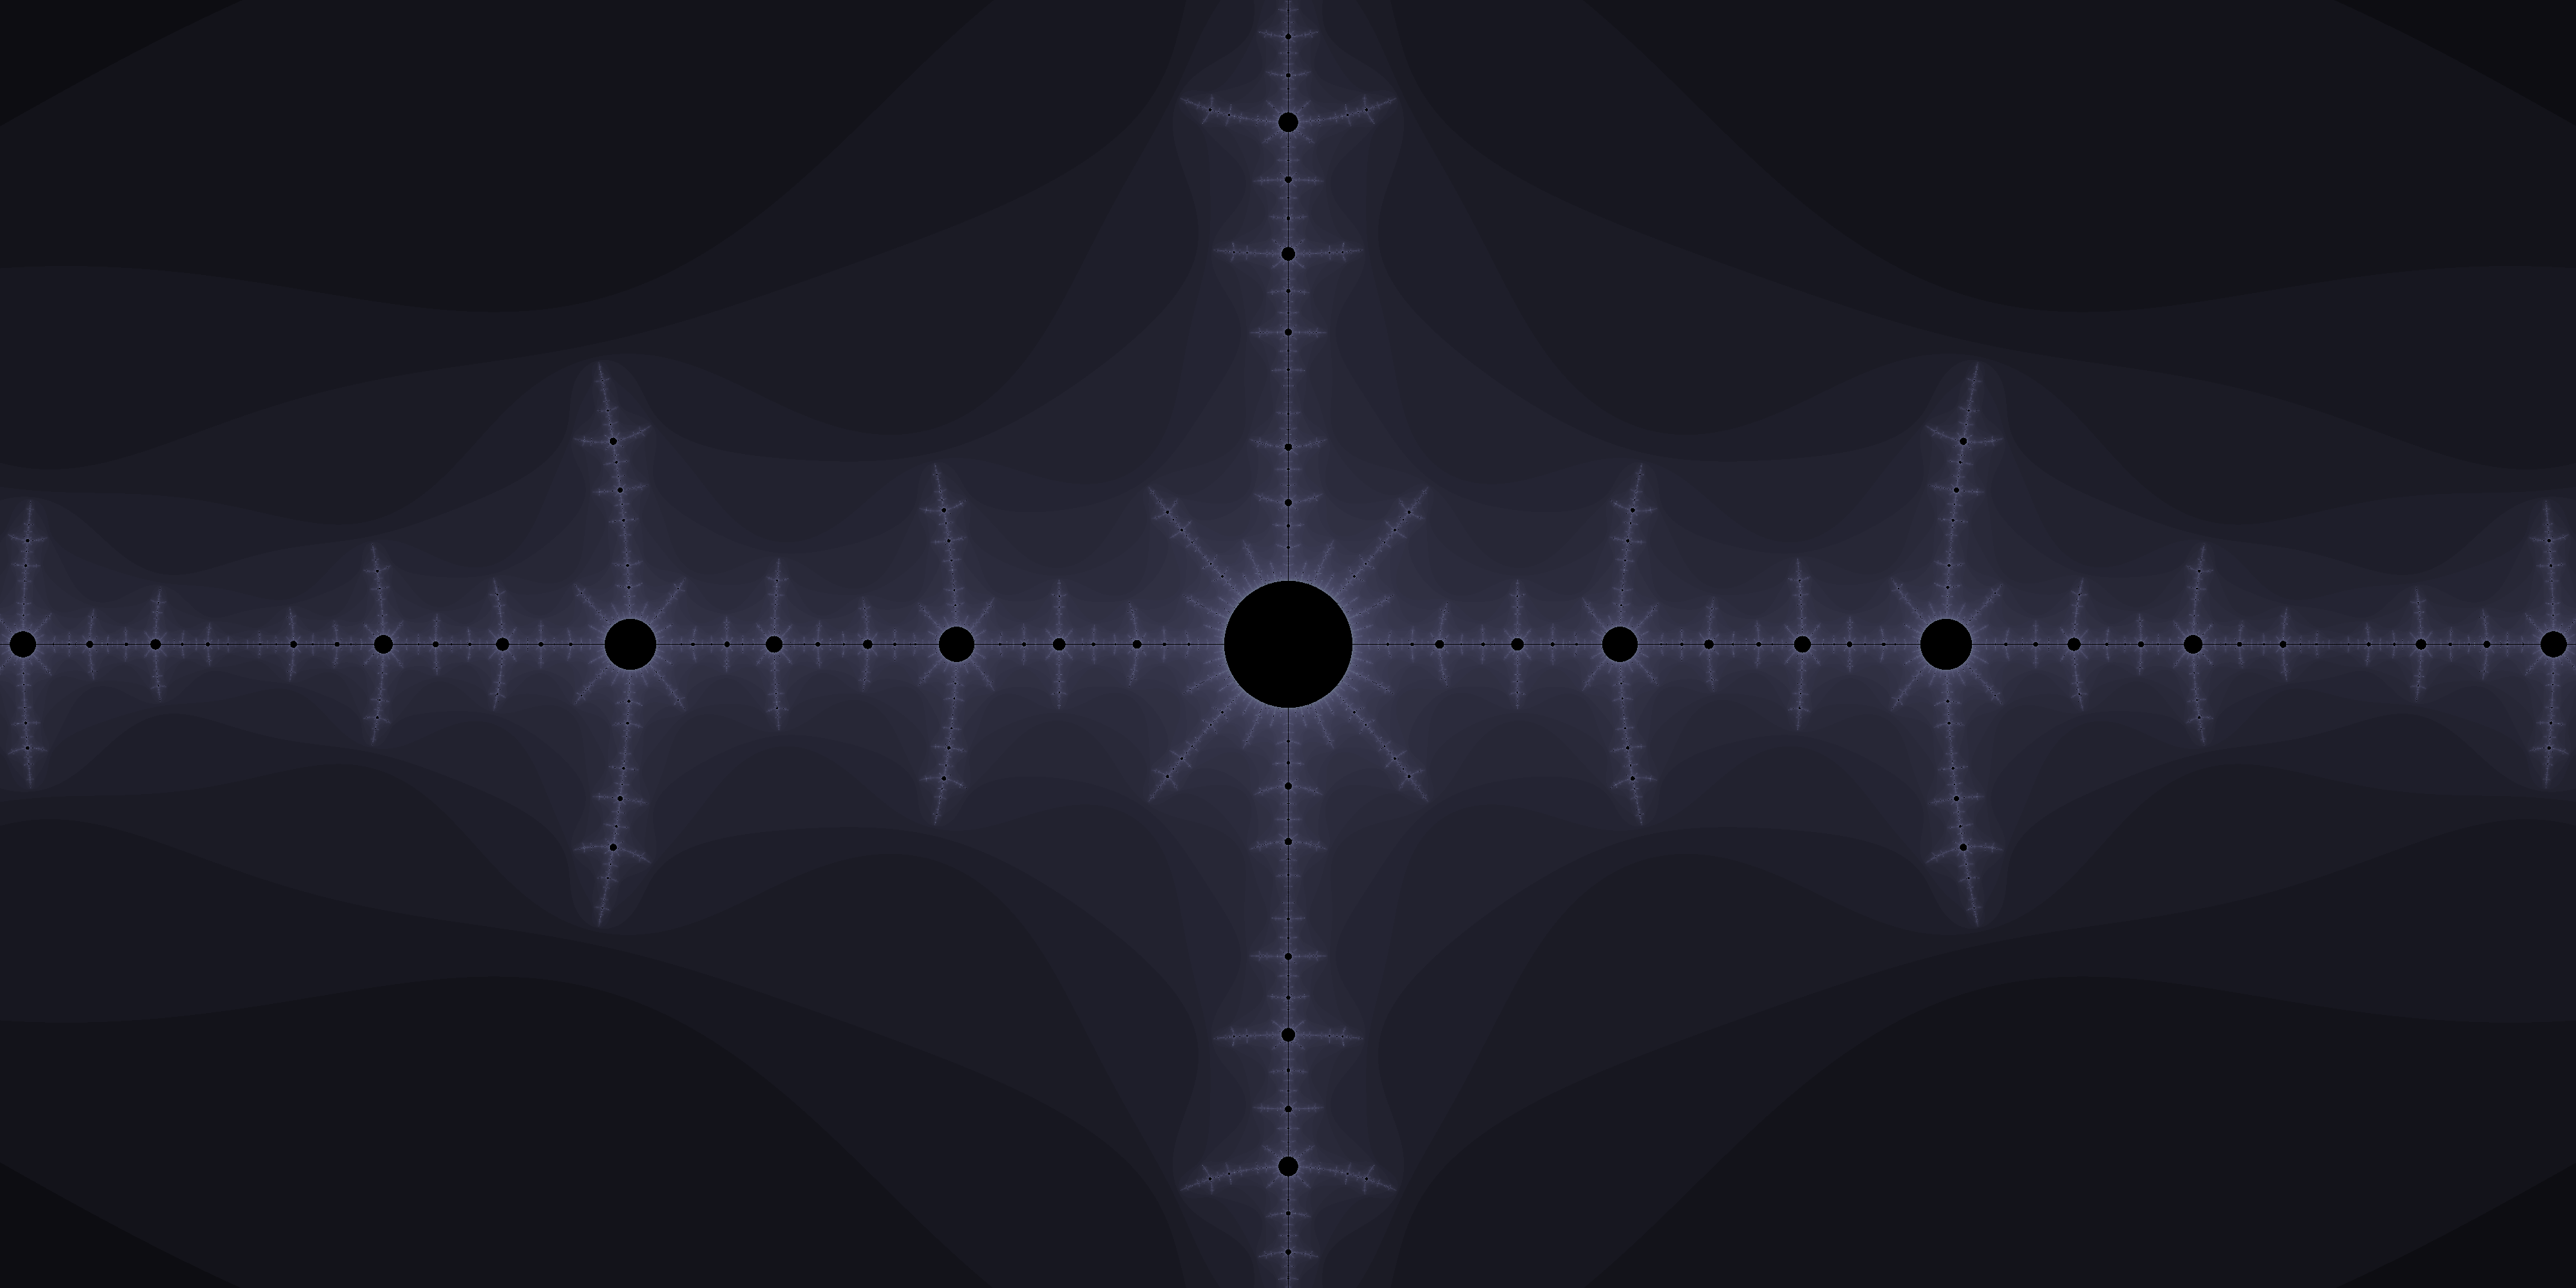
\includegraphics[width=\linewidth]{Utils/article_dependencies/Honorable_mentions/2.png}
\end{figure}

\begin{figure}[H]
	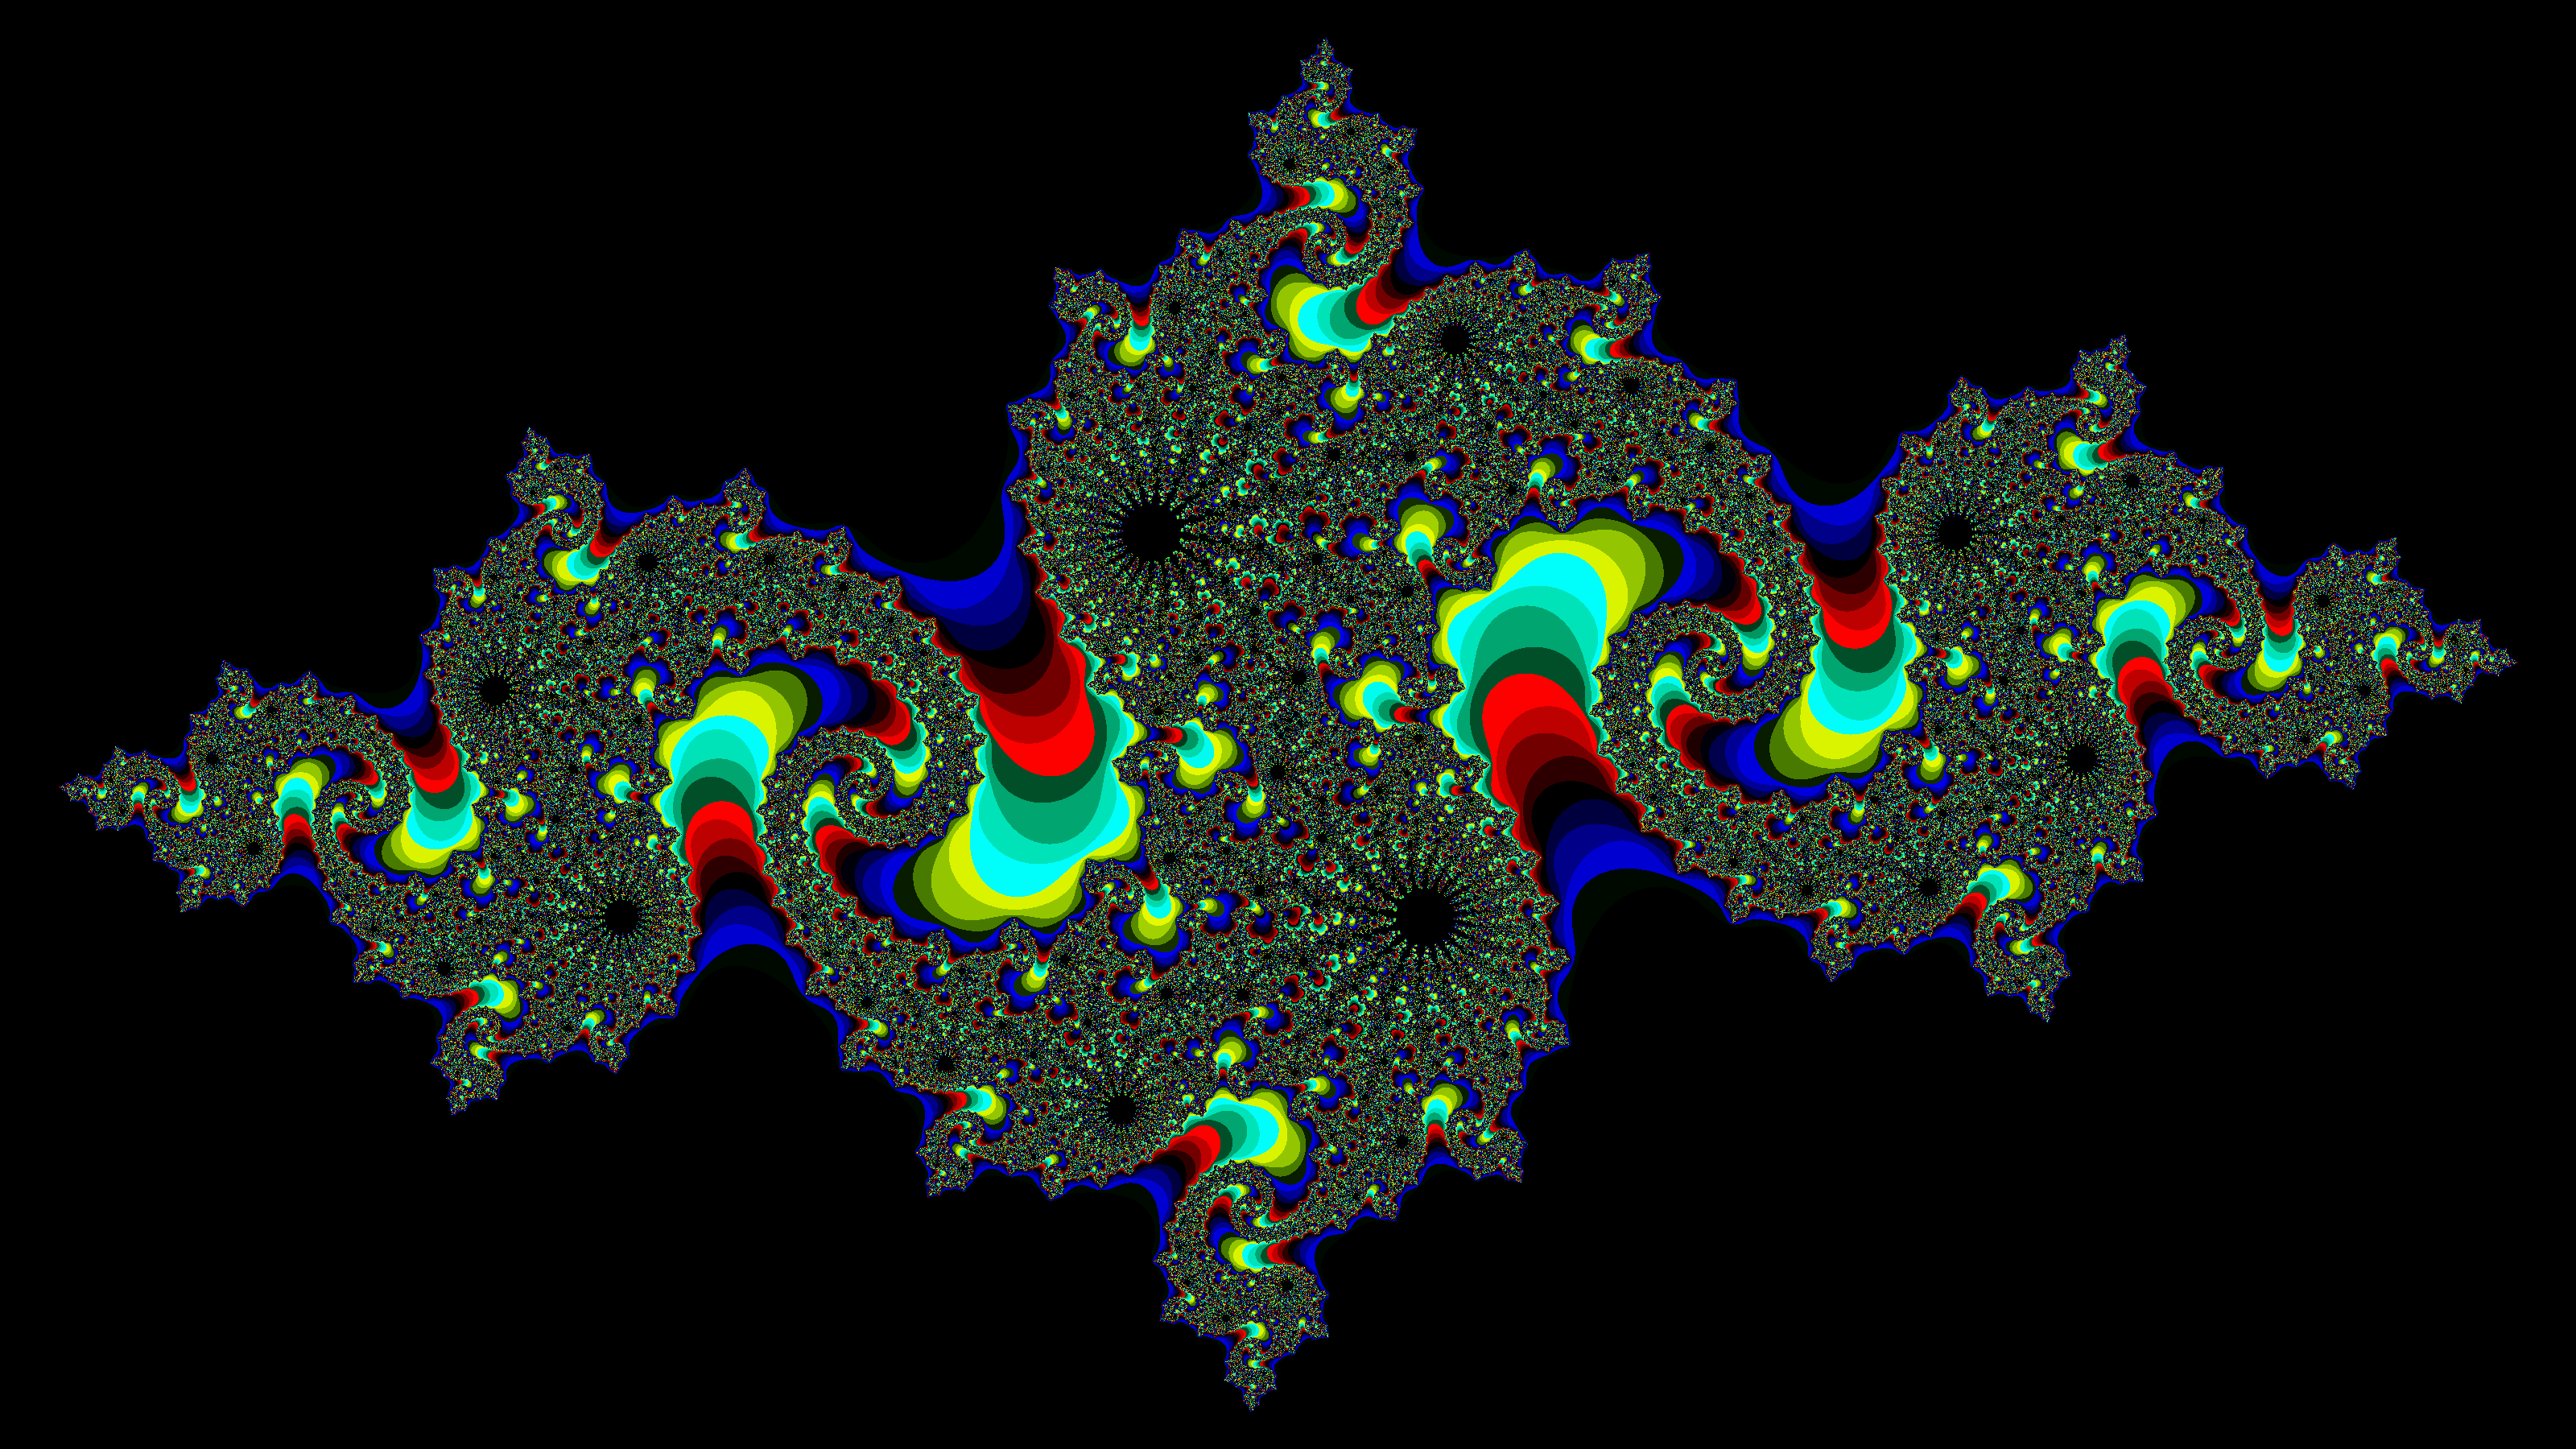
\includegraphics[width=\linewidth]{Utils/article_dependencies/Honorable_mentions/3.png}
\end{figure}

\begin{figure}[H]
	\includegraphics[width=\linewidth]{Utils/article_dependencies/Honorable_mentions/4.png}
\end{figure}

\begin{figure}[H]
	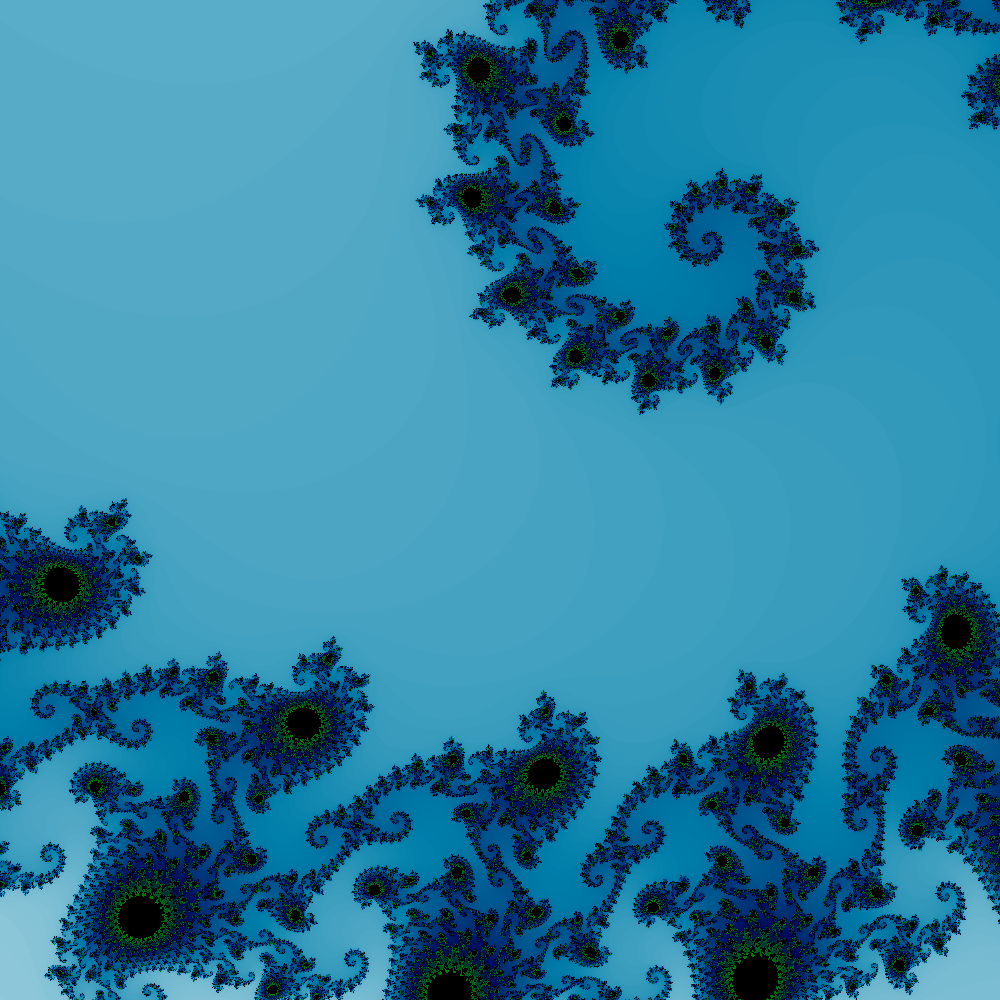
\includegraphics[width=\linewidth]{Utils/article_dependencies/Honorable_mentions/5.png}
\end{figure}

\begin{figure}[H]
	\includegraphics[width=\linewidth]{Utils/article_dependencies/Honorable_mentions/6.png}
\end{figure}

\begin{figure}[H]
	\includegraphics[width=\linewidth]{Utils/article_dependencies/Honorable_mentions/7.png}
\end{figure}

\begin{figure}[H]
	\includegraphics[width=\linewidth]{Utils/article_dependencies/Honorable_mentions/8.png}
\end{figure}

\begin{center}
	\footnotesize
	\href{run:Utils/article_dependencies/Implementation_chapter/render_10.gif}{Psychodelic effect obtained by shifting color mapping each frame}
\end{center}

\pagebreak
\printbibliography[heading=bibintoc, title={References}]
\end{document}